\documentclass[12pt]{scrartcl}
\usepackage{datetime}
\title{Report\\Homework 6}
\author{Dheeraj Kumar Pant\\19111029 \and Jay Raj Singh\\19111038 \and Anurag Maithani\\19111015}
\usepackage{amsmath}
\usepackage{amssymb}
\usepackage{graphicx}
\usepackage{array}

\begin{document}
\maketitle
\hfill \break
\\
\\
\\
In this assignment we have data with stressed grid condition(denoted by label 1) and normal grid condition(denoted by label 0). Since we have to do unsupervised learning , so we have dropped the label from our dataset. After that we have performed clustering on various forms of this resultant dataset which we got after removing the labels. We have projected this dataset in diffusion space and  done clustering in diffusion space with original dimensions as well as in reduced dimension. For dimensionlity reduction we have used two methods first one is from paper covered in class and the second one is Singular Value Decomposition. Here for plots Label 0 is represented by blue dots and Label 1 is represented by Red. Below is 3D plot for original data points in reduced dimensions. Here in below figure we have used singular value decomposition to reduce its dimensionality to three. 
\begin{figure}[h]
    		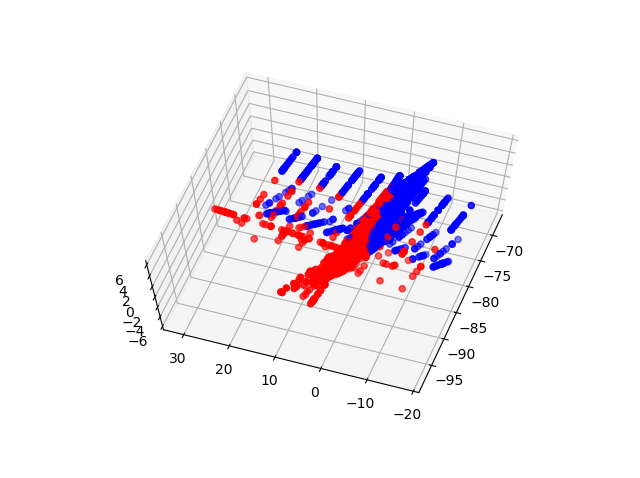
\includegraphics[scale=0.5]{Original_data_.png}
    		\includegraphics[scale=0.5]{Original_data.png}
    		
\end{figure}
\newpage
Below are three dimensional plots and scree plot of Data Matrix in diffusion space with its dimensionality reduced to 3. We have taken best three cases which we got from different values of sigma and diffusion steps
\begin{figure}[h]
\textbf{A.\quad Plots for \textit{sigma = 1} and \textit{diffusion steps(t) = 10}}
\\\\
In this case we get clustering results as: \textbf{(4117,33)}. From the below plots it is clear that the data orientation is worst in this case.\\    		
    		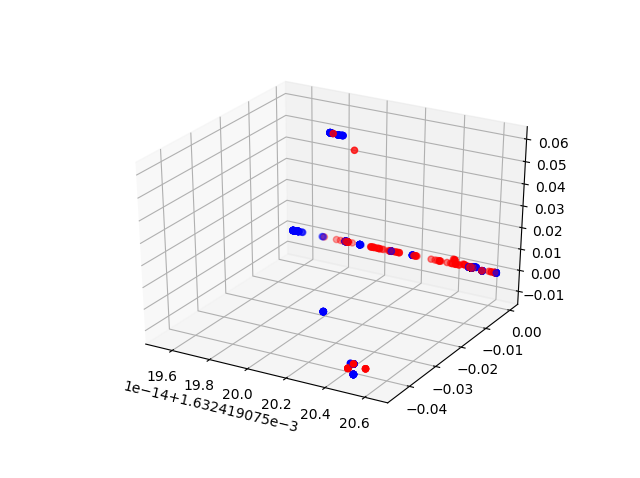
\includegraphics[scale=0.5]{1_10.png}
    		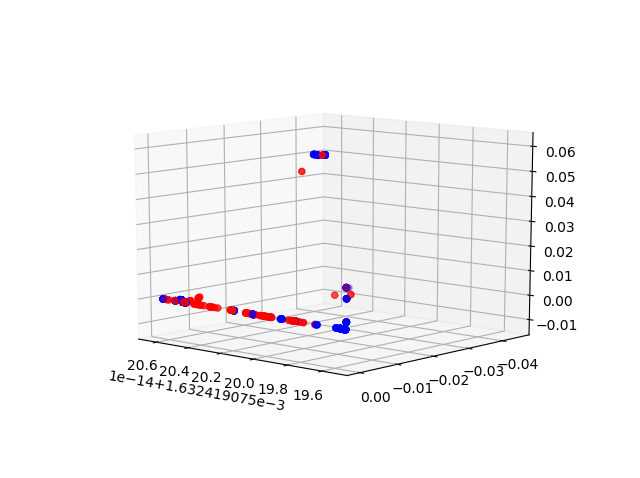
\includegraphics[scale=0.5]{1_10_.png}
    		
\end{figure}
\begin{figure}[h]
    		
    		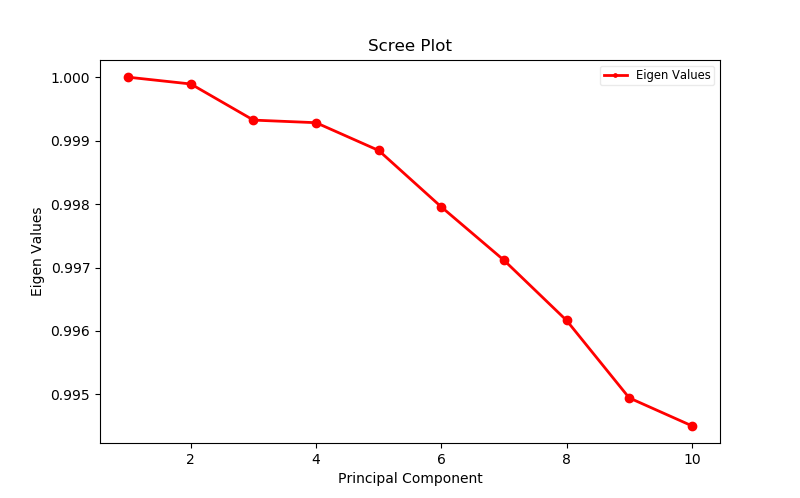
\includegraphics[scale=0.5]{1_10_S.png}
    		
\end{figure}
\newpage
\begin{figure}[h]
\textbf{B.\quad Plots for \textit{sigma = 5} and \textit{diffusion steps(t) = 10}}
\\\\
In this case we get clustering results as: \textbf{(4013,137)}. This is slightly better than the previous one but from the below plots it is clear that this case has no better answer.\\    		
    		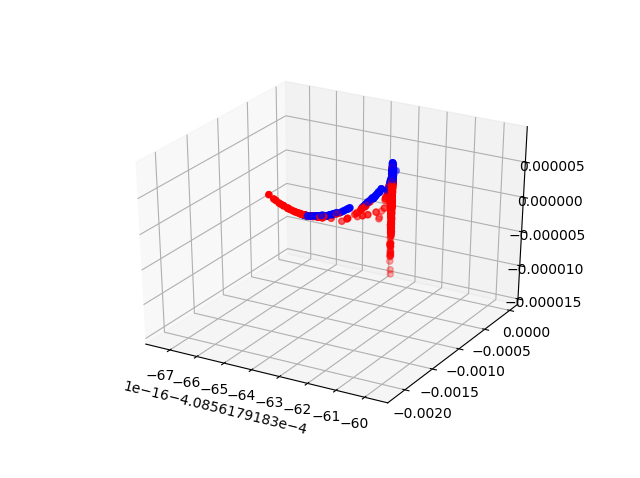
\includegraphics[scale=0.5]{5_10.png}
    		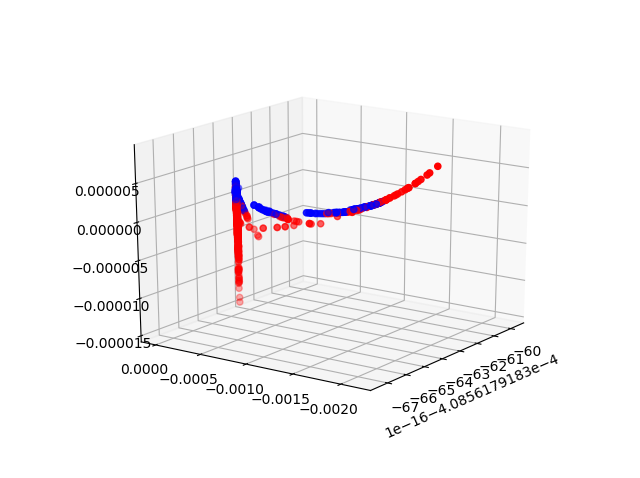
\includegraphics[scale=0.5]{5_10_.png}
    		
\end{figure}
\begin{figure}[h]
    		
    		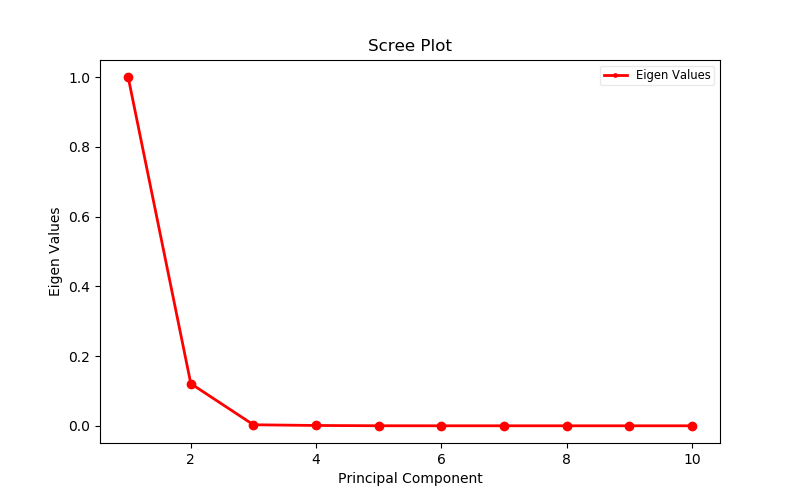
\includegraphics[scale=0.5]{5_10_S.png}
    		
\end{figure}
\newpage
\begin{figure}[h]
\textbf{C.\quad Plots for \textit{sigma = 2} and \textit{diffusion steps(t) = 20}}
\\\\
In this case we get clustering results as: \textbf{(3914,236)}. This is slightly better than the previous one but will never be able to defeat the orientation of original data itself.\\
		
    		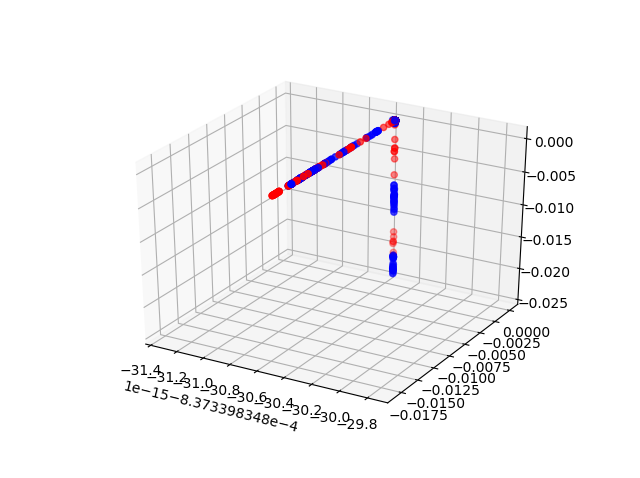
\includegraphics[scale=0.5]{2_20_.png}
    		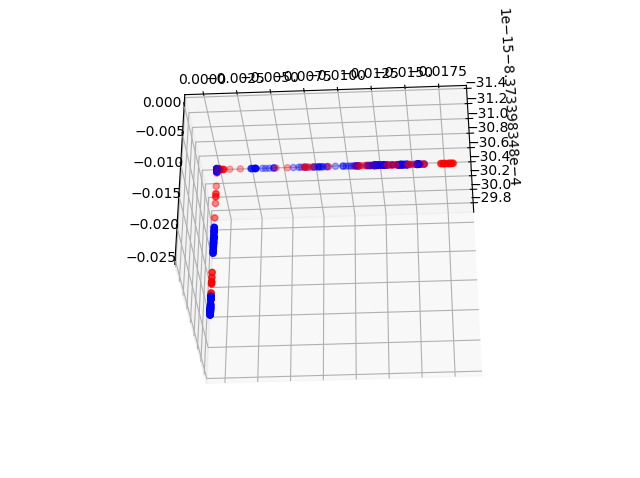
\includegraphics[scale=0.5]{2_20__.png}
    		
\end{figure}
\begin{figure}[h]
    		
    		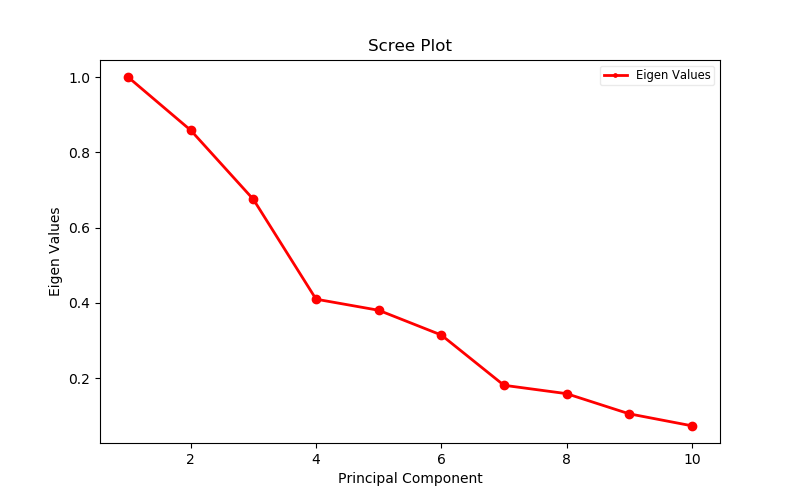
\includegraphics[scale=0.5]{2_20.png}
    		
\end{figure}
\newpage
{\Large{\textbf{CONCLUSION}}}\\\\
Clustering stats after applying KMeans directly on the original data are (1009,3141), which is very much better than the statistics shown in above cases.
So at last we concluded that in our data-set diffusion map doesn't work. We are getting worst orientation of data after mapping to diffusion space and thus worst clustering. Our data seems to be oriented in better way originally and hence euclidean distance in original space will work fine in our data-set, hence no need to apply diffusion map. 
\end{document} 